%% LyX 2.3.3 created this file.  For more info, see http://www.lyx.org/.
%% Do not edit unless you really know what you are doing.
\documentclass[10pt]{article}
\usepackage{ae,aecompl}
\usepackage[T1]{fontenc}
\usepackage[utf8]{inputenc}
\usepackage{geometry}
\geometry{verbose,tmargin=2cm,bmargin=2cm,lmargin=2cm,rmargin=2cm} %biorxiv version
%\geometry{verbose,footskip=0.75in}
\usepackage{color}
%\usepackage{float}
\usepackage{url}
\usepackage{amsmath}
\usepackage{amssymb}
\usepackage{graphicx}
\usepackage{authblk}
\usepackage{natbib}
\usepackage{microtype}
\usepackage[unicode=true,
 bookmarks=false,
 breaklinks=false,
 pdfborder={0 0 1},
% backref=section,
 colorlinks=true]
 {hyperref}
\hypersetup{
 allcolors=blue}
 
 %Only to be able to strike text out, to make it more visible
\usepackage{cancel}

\makeatletter
%%%%%%%%%%%%%%%%%%%%%%%%%%%%%% Textclass specific LaTeX commands.
\newcommand{\lyxaddress}[1]{
	\par {\raggedright #1
	\vspace{1.4em}
	\noindent\par}
}

%%%%%%%%%%%%%%%%%%%%%%%%%%%%%% User specified LaTeX commands.
% line numbers
\usepackage{lineno}
%Spacing will be better
\usepackage{setspace}

\makeatother

\renewcommand*{\Affilfont}{\normalsize}
\title{Strong self-regulation and widespread facilitative interactions in phytoplankton communities}
%\author{Coralie Picoche\textsuperscript{1,2}, Frédéric Barraquand\textsuperscript{1,2{*}}}
\author[1,2]{Coralie Picoche}
\author[1,2,*]{Frédéric Barraquand}
\affil[1]{Integrative and Theoretical Ecology, LabEx COTE, University of Bordeaux, Pessac, France}
\affil[2]{Institute of Mathematics of Bordeaux, CNRS, University of Bordeaux, Talence, France}
\setlength{\affilsep}{2em}  
\date{}

\begin{document}
\onehalfspacing
\maketitle
\thispagestyle{empty}
%\doublespacing\bigskip{} % for the article
%biorxiv

%\lyxaddress{1 -- University of Bordeaux, Integrative and Theoretical Ecology, LabEx COTE, Bât. B2 - Allée Geoffroy St-Hilaire, 33615 Pessac, France}
%\lyxaddress{2 -- CNRS, Institute of Mathematics of Bordeaux, 351 Cours de la Libération, 33405 Talence, France}
% For J Ecol  Correspondence: Frédéric Barraquand, CNRS, Institute of Mathematics of Bordeaux, 351 Cours de la Libération, 33405 Talence, France}
%\textbf{{*}}frederic.barraquand@u-bordeaux.fr;

%\newpage{}

\section*{Abstract}

\begin{enumerate}
\item The persistence of phytoplanktonic diversity in spite of competition
for basic resources has long been a source of wonder and inspiration
to ecologists. To sort out, among the many coexistence mechanisms
suggested by theory and experiments, which ones actually maintain
diversity in natural ecosystems, long-term field studies are paramount. 
\item We analysed a large dataset of phytoplankton abundance time series
using dynamic, multivariate autoregressive models. Phytoplankton was
counted and identified down to the genus level, every two weeks over
twenty years, at ten sites along the French coastline. Multivariate
autoregressive models allowed to estimate biotic interaction networks,
while also accounting for abiotic variables that may drive part of
the phytoplankton fluctuations. We then analysed the ratio of intra-
to inter-taxa interactions (measuring self-regulation, itself a measure
of niche differentiation), the frequency of negative vs positive interactions,
and how stability metrics (both at the network and genus level) relate
to network complexity and genus self-regulation or abundance. 
\item We showed that a strong self-regulation, with competition strength
within a taxon (genus) an order of magnitude higher than between taxa,
was present in all phytoplanktonic interaction networks. This much
stronger intragenus competition suggests that niche differentiation
- rather than neutrality - is commonplace in phytoplankton. Furthermore,
interaction networks were dominated by positive net effects between
phytoplanktonic taxa (on average, more than 50\% of interactions were positive).
While network stability (\textit{sensu} resilience) was unrelated
to complexity measures, we unveiled links between self-regulation,
intergenus interaction strengths and abundance. The less common taxa
tend to be more strongly self-regulated and can therefore maintain
in spite of competition with more abundant ones. 
\item \textit{Synthesis}: We demonstrate that strong niche differentiation, widespread
facilitation between phytoplanktonic taxa and stabilizing covariances
between interaction strengths should be common features of coexisting
phytoplankton communities in the field. These are structural properties
that we can expect to emerge from plausible mechanistic models of
phytoplankton communities. We discuss mechanisms, such as predation
or restricted microscale movement, that are consistent with these
findings, which paves the way for further research.
\end{enumerate}
\textbf{Keywords}: phytoplankton; coexistence; facilitation; mutualism;
niche theory; time series; networks
\let\thefootnote\relax\footnotetext{* Correspondence: frederic.barraquand@u-bordeaux.fr} % for biorxiv

%\linenumbers 
% % for biorxiv

\newpage{}

\doublespacing % for biorxiv

\section*{Introduction}

How species or close genera can coexist together in spite of competition
is one of the main puzzles of community ecology, especially for primary
producers that seemingly share the same basic resources \citep{hutchinson_paradox_1961}.
Many theoretical studies of competition models have shown that competitive
exclusion is likely in those circumstances, unless mechanisms involving
spatial or temporal variation are at play \citep{armstrong1976coexistence,armstrong1980competitive,chesson_roles_1997,huisman_biological_2001,li_effects_2016,chesson_updates_2018}.
Neutral theory, assuming that all individuals have equal birth and death rates and exert equal competitive pressure on conspecifics and heterospecifics alike, produces a non-equilibrium coexistence maintained by dispersal from a regional pool. It has been proposed as a solution to the puzzle presented by highly diverse communities \citep{hubbell_unified_2001,rosindell2011unified}. 
%Neutral theory, that assumes a non-equilibrium coexistence maintained by dispersal and equal competitive abilities for all species (\citealt{hubbell_unified_2001}, though there are exceptions, see \citealt{volkov_neutral_2003,volkov_patterns_2007}), has been proposed as a solution to explain highly diverse communities \citep{hubbell_unified_2001,rosindell2011unified}.

However, the evidence gathered from terrestrial plant communities
starts to suggest that, in fact, niche rather than neutral processes
may be paramount to explain coexistence, with intraspecific competition
dwarfing interspecific competition in most cases \citep{adler_coexistence_2010,adler_competition_2018}; see also \citet{volkov_patterns_2007,volkov_inferring_2009}.
Whether these conclusions drawn mostly from studies of terrestrial
plants apply to other ecosystems and taxa is currently little known
(but see \citealt{mutshinda_what_2009}).

Moreover, competition may not be the rule: the meta-analysis by \citet{adler_competition_2018}
reported a large number of facilitative interactions (30\%) and several
reviews \citep{brooker_facilitation_2008,mcintire2014facilitation,kinlock_meta-analysis_2019}
have highlighted that facilitation may be much more widespread than
ecologists usually tend to think. Although some theoretical studies
suggest that facilitative interactions can be destabilizing (\emph{sensu}
resilience) and therefore undermine coexistence in Lotka-Volterra
models \citep{coyte_ecology_2015}, multiple other modelling \citep{gross_positive_2008}
and empirical \citep{brooker_facilitation_2008,cavieres2009facilitative}
studies have suggested that facilitative interactions can to a large
degree benefit coexistence, especially when multiple interaction types
are considered simultaneously \citep{mougi2012diversity,garcia2018effect}.

Here, we analyse a spatially replicated, long-term community-level
dataset, consisting of ten multivariate time series of phytoplankton
abundance along the French coastline. We do so 
using multivariate autoregressive (MAR) models, that allow to estimate interactions
between genera. Although many ecological studies focus on interactions
between species, competition has been shown experimentally to occur
between different genera of phytoplankton \citep{titman_ecological_1976,descamps-julien_stable_2005}.
The genus level is also a rather fine taxonomic scale for phytoplankton
interaction studies, as most studies are restricted to interactions
between different classes or even phyla \citep{ives_estimating_2003,hampton_sixty_2008,griffiths_phytoplankton_2015}.
Studying interactions between different genera of phytoplankton therefore
both makes empirical sense in light of competition experiments and
allows to estimate better-resolved networks. We focus here on genera
that belong mostly to diatoms and dinoflagellates. To put our results
into a more general context, we then compare our interaction strength
estimates to previously published interaction networks produced under
the same statistical framework, both in plankton and other empirical
systems.

\section*{Material and methods}

\subsection*{Sampling methods}

All phytoplankton samples were collected by Ifremer coastal laboratories
as part of the National Phytoplankton and Phycotoxin Monitoring Network
\citep{REPHY_db}. Since 1987, this monitoring program has required
the sampling of 26 sites along the French coastline every 2 weeks
within 2 hours of high tide to document both biotic (phytoplankton
counts) and abiotic (water temperature, salinity) variables. We focused
on sites which had the longest time series. We also excluded time
series which had missing data for over 6 months or an average delay
between sampling dates above 20 days. This reduced the number of study
sites to 10 sites nested within 4 regions (Brittany, Oléron, Arcachon
and the Mediterranean Sea; Fig.~S1 and Table S1 in the Supporting Information).

Abiotic variables (temperature, salinity) were measured directly from
the boat during the sampling process while water samples for biotic
analyses were fixed with a Lugol's solution and examined later. Phytoplankton
cells above 20 $\mu$m were identified at the lowest possible taxonomic
level and counted with the Utermöhl method using an optical microscope
\citep{utermohl_zur_1958}. Throughout the years and sites, more than
600 taxa were identified at different taxonomic levels. We aggregated
them at the genus (or group of genera when not possible) level based
on previous work (Table S2; \citealt{hernandez_farinas_assessing_2015,barraquand_coastal_2018}),
except for cryptophytes and euglenophytes in Arcachon, which could
not be identified below the family level. Although the taxonomic resolution
used here may seem coarse in comparison to land plants, it is in fact
more refined than 86\% of the MAR(1) studies of phytoplankton listed
in Table~S4.

For each region, the MAR(1) analysis focused on the most abundant
and most frequently observed genera to avoid most of the gaps in the
time series. When gaps did not
exceed a month, missing values were linearly interpolated; remaining
missing values were replaced by a random number between 0 and half
of the lowest observed abundance \citep{hampton_coalescence_2006}. Time series are plotted in Fig. S2. 
We tested extensively this and other methods to deal with missing
data in a previous publication on a subset of this dataset \citep{barraquand_coastal_2018}.
All time series were scaled and centered before MAR analyses.

\subsection*{MAR(1) model}

Multivariate autoregressive (MAR) models are used to determine the
interspecific interactions and abiotic effects shaping a community's
dynamics \citep{ives_estimating_2003}. MAR(1) models are based on
a stochastic, discrete-time Gompertz equation which relates the log-abundance
of each of the $S$ taxa at time $t+1$ to log-abundances of the whole
community at time $t$, with possible interactions between taxa, and
effects of $V$ abiotic variables at time $t+1$. These assumptions
are encapsulated in eq.~\ref{eq:MAR}:

\begin{equation}
\mathbf{n}_{t+1}=\mathbf{B}\mathbf{n}_{t}+\textbf{C}\textbf{u}_{t+1}+\mathbf{e}_{t},\mathbf{e}_{t}\thicksim\mathcal{{N_{S}}}(0,\mathbf{Q})\label{eq:MAR}
\end{equation}

where $\mathbf{n}_{\ensuremath{t}}$ is the $1\times S$ vector of
log-abundance of phytoplankton taxa, $\mathbf{B}$ is the $S\times S$
community (interaction) matrix, $\mathbf{C}$ is the $S\times V$
environment matrix describing the effects of $V$ variables (stacked
in vector $\mathbf{u}_{t+1}$) on growth rates, with $V=2$ in our
case (temperature and salinity). The noise $\mathbf{e}_{t}$ is a
$1\times S$ noise vector, following a multivariate normal distribution with a variance-covariance
matrix $\mathbf{Q}$. $\mathbf{Q}$ is diagonal and we have previously
showed that this parsimonious choice did not affect qualitatively
the results \citep{barraquand_coastal_2018}. We used the MARSS package
\citep{holmes_analysis_2014} v3.9, in R v3.3.2 \citep{venables_r_2013},
to estimate parameters with a maximum likelihood procedure.

Our previous analysis of the Arcachon region, for which more covariables
were available \citep{barraquand_coastal_2018}, revealed that hydrodynamics
and hydrology had more influence on phytoplankton dynamics than nutrients
on the two-week timescale. Because temperature and salinity sum up
seasonal changes in light as well as hydrology (salinity is inversely
related to freshwater inflow), these represent the two key drivers
needed to account for abiotic influences \citep{scheef_inferring_2013}.
They are therefore used to summarize the abiotic environment in the
remainder of the article.

The analysis of real data in \citet{barraquand_coastal_2018} was
complemented by that of simulated data mimicking the study design,
which confirmed the ability of MAR(1) models to infer biotic interactions
and abiotic forcings. Fitting a more sophisticated model (threshold
autoregressive model) did not reveal extra non-linearities or a storage
effect in the Arcachon subset of the data \citep{barraquand_coastal_2018}.
Other aspects of the MAR(1) modelling are likewise quite robust: using
two abiotic variables (temperature and salinity) in this study rather
than the full set used in \citet{barraquand_coastal_2018} led to
almost identical covariate effects and interaction estimates for the
Arcachon study sites. Even if some departures from the true data-generating
model may not always be detectable through MAR(1) diagnostics (e.g.,
residuals), the analysis of nonlinear simulations has showed that
MAR(1) models are in general robust to nonlinearities if the inference
focuses on interaction sign and order of magnitude of model coefficients
\citep{certain_how_2018}, which is how these models are used here. For ease of interpretation of MAR(1) interaction coefficients, we also highlight how intra- and inter-taxa interaction strengths in a MAR(1) model map to their counterparts in a multispecies Beverton-Holt model, i.e., a discrete-time Lotka-Volterra model \citep{cushing_discrete_2004}, in the Supporting Information.

In this study, the number of phytoplankton taxa ($S$) and the community
composition vary slightly between regions but sites share on average
67\% of their taxa. In order to have comparable models, we also keep
the same 2 covariates, i.e., water temperature and salinity, that
were measured at all study sites. Therefore, the dimension of the
dynamical system depends on the (square of the) number of phytoplankton
taxa we study, which ranges between 7 (Mediterranean Sea) and 14 (Brittany).
The smallest system still requires 63 parameters to be estimated (49
for the $7\times7$ interaction matrices and 14 for the $7\times2$
environment matrices) if we consider all possible interactions between
taxa. To reduce this dimensionality and remove unnecessary parameters,
we built different `interaction scenarios' based on known phylogenetic
information \citep[as suggested in][]{violle_phylogenetic_2011,narwani_ecological_2017}.
The null interaction scenario assumed no interaction between genera
(diagonal interaction matrix) and was compared to four other interaction
scenarios. The first interaction scenario assumed that interactions
could only occur between phylogenetically close organisms, i.e., within
a class (groups were then diatoms, dinoflagellates, and other phytoplanktonic
organisms) while the second interaction scenario further differentiated
pennate and centric diatoms. The third interaction scenario considered
the reverse hypothesis, that only unrelated organisms could interact
(i.e., a diatom could only interact with a dinoflagellate or a cryptophyte,
but not with another diatom), and the last interaction scenario did
not constrain the interactions at all (full interaction matrix). We
selected the best scenario by comparing BIC (Fig.~S3), which proved
to be satisfactory in our previous analyses of both real data and
similar simulated datasets (\citealp{barraquand_coastal_2018}, Appendix
2). The second interaction scenario, hereafter called the pennate-centric
scenario, had the lowest BIC for all sites (Fig. S3). This parsimonious
scenario was therefore chosen as the basis for further investigations
of network structure.

\subsection*{Analysis of interaction strengths}

The interaction matrix obtained from MAR(1) analyses can be used to
determine the stability of a discrete-time dynamical system \citep{ives_stability_1999,ives_estimating_2003}. 
To investigate stability-complexity relationships, we compared the maximum modulus of the eigenvalues of the pennate/centric
matrices for each site to network descriptors. The maximum modulus is analogous
to the real part of the leading eigenvalue for continuous time models,
and measures resilience while still accounting for some variability
properties \citep{ives_stability_1999}. However, because most theory on stability-complexity has been developed in continuous time \citep[e.g.,][]{allesina_stabilitycomplexity_2015}, we numerically checked that the maximum modulus of the eigenvalues in a discrete-time interaction matrix and its continuous-time model counterpart yield similar information in the Supporting Information. We then compared this resilience measure to complexity metrics, such as the interaction strength distribution (sign, mean and variance) and weighted connectance \citep{bersier_quantitative_2002}. Weighted connectance is a
measure of the proportion of realized links compared to all possible
links, taking into account the shape of the flux distribution. This
metric is adapted to weighted interaction matrices but cannot accommodate
for both positive and negative coefficients: we therefore chose to
focus on interaction strength only (absolute values of the coefficients),
irrespective of interaction sign. In contrast, mean and variance of
the off-diagonal coefficients, which can affect the stability of a
community \citep{allesina_stabilitycomplexity_2015}, are computed
on raw values of the coefficients. Interaction coefficient variance is multiplied by the number of taxa, according to theory \citep{allesina_stabilitycomplexity_2015}.

In addition to these network-level metrics, we also computed the average
vulnerability (average effect of other taxa on a focal taxon, eq.~S5)
and impact (average effect of a focal taxon on other taxa, eq.~S6)
on both raw and absolute values of the coefficients. Vulnerability
and impact can be related to in-strength and out-strength in the meta-analysis
of \citet{kinlock_meta-analysis_2019}. We then compared these to
the regulation a focal species exerted on itself. Raw values indicate
the average effect that can be expected on the growth rate of a taxon
from the rest of the community (i.e., is the effect of others mostly
positive or negative?), while absolute effects characterise the strength
of all types of interactions on a taxon (i.e., is a taxon strongly
affected by the others?).

Finally, we compared the observed ratio between mean self-regulation
(intrataxon interaction strength) and mean intertaxa interaction strength
to other published studies based on a MAR(1) model. A list of references
is given in Table~S4. Authors usually reported only coefficients
that were significant with a 5\% significance level, thus ignoring
potentially many weak effects, which we had to set to 0. There are
therefore two ways of computing the mean intertaxa interactions, i.e.,
taking the mean value of all coefficients outside of the matrix diagonal,
including zeroes (which decreases the estimated mean intertaxa interaction
strength, Fig. \ref{fig:meta_ratio}), or taking the mean value of
statistically significant intertaxa coefficients only (which increases
the estimated mean intertaxa interaction strength, Fig. S9). We considered
both; a detailed description of these different ways to compare intra- and inter-taxa interactions can be found in the Supporting Information.

\section*{Results}

\subsection*{Interaction estimates}

\begin{figure}[!ht]
\centering 
%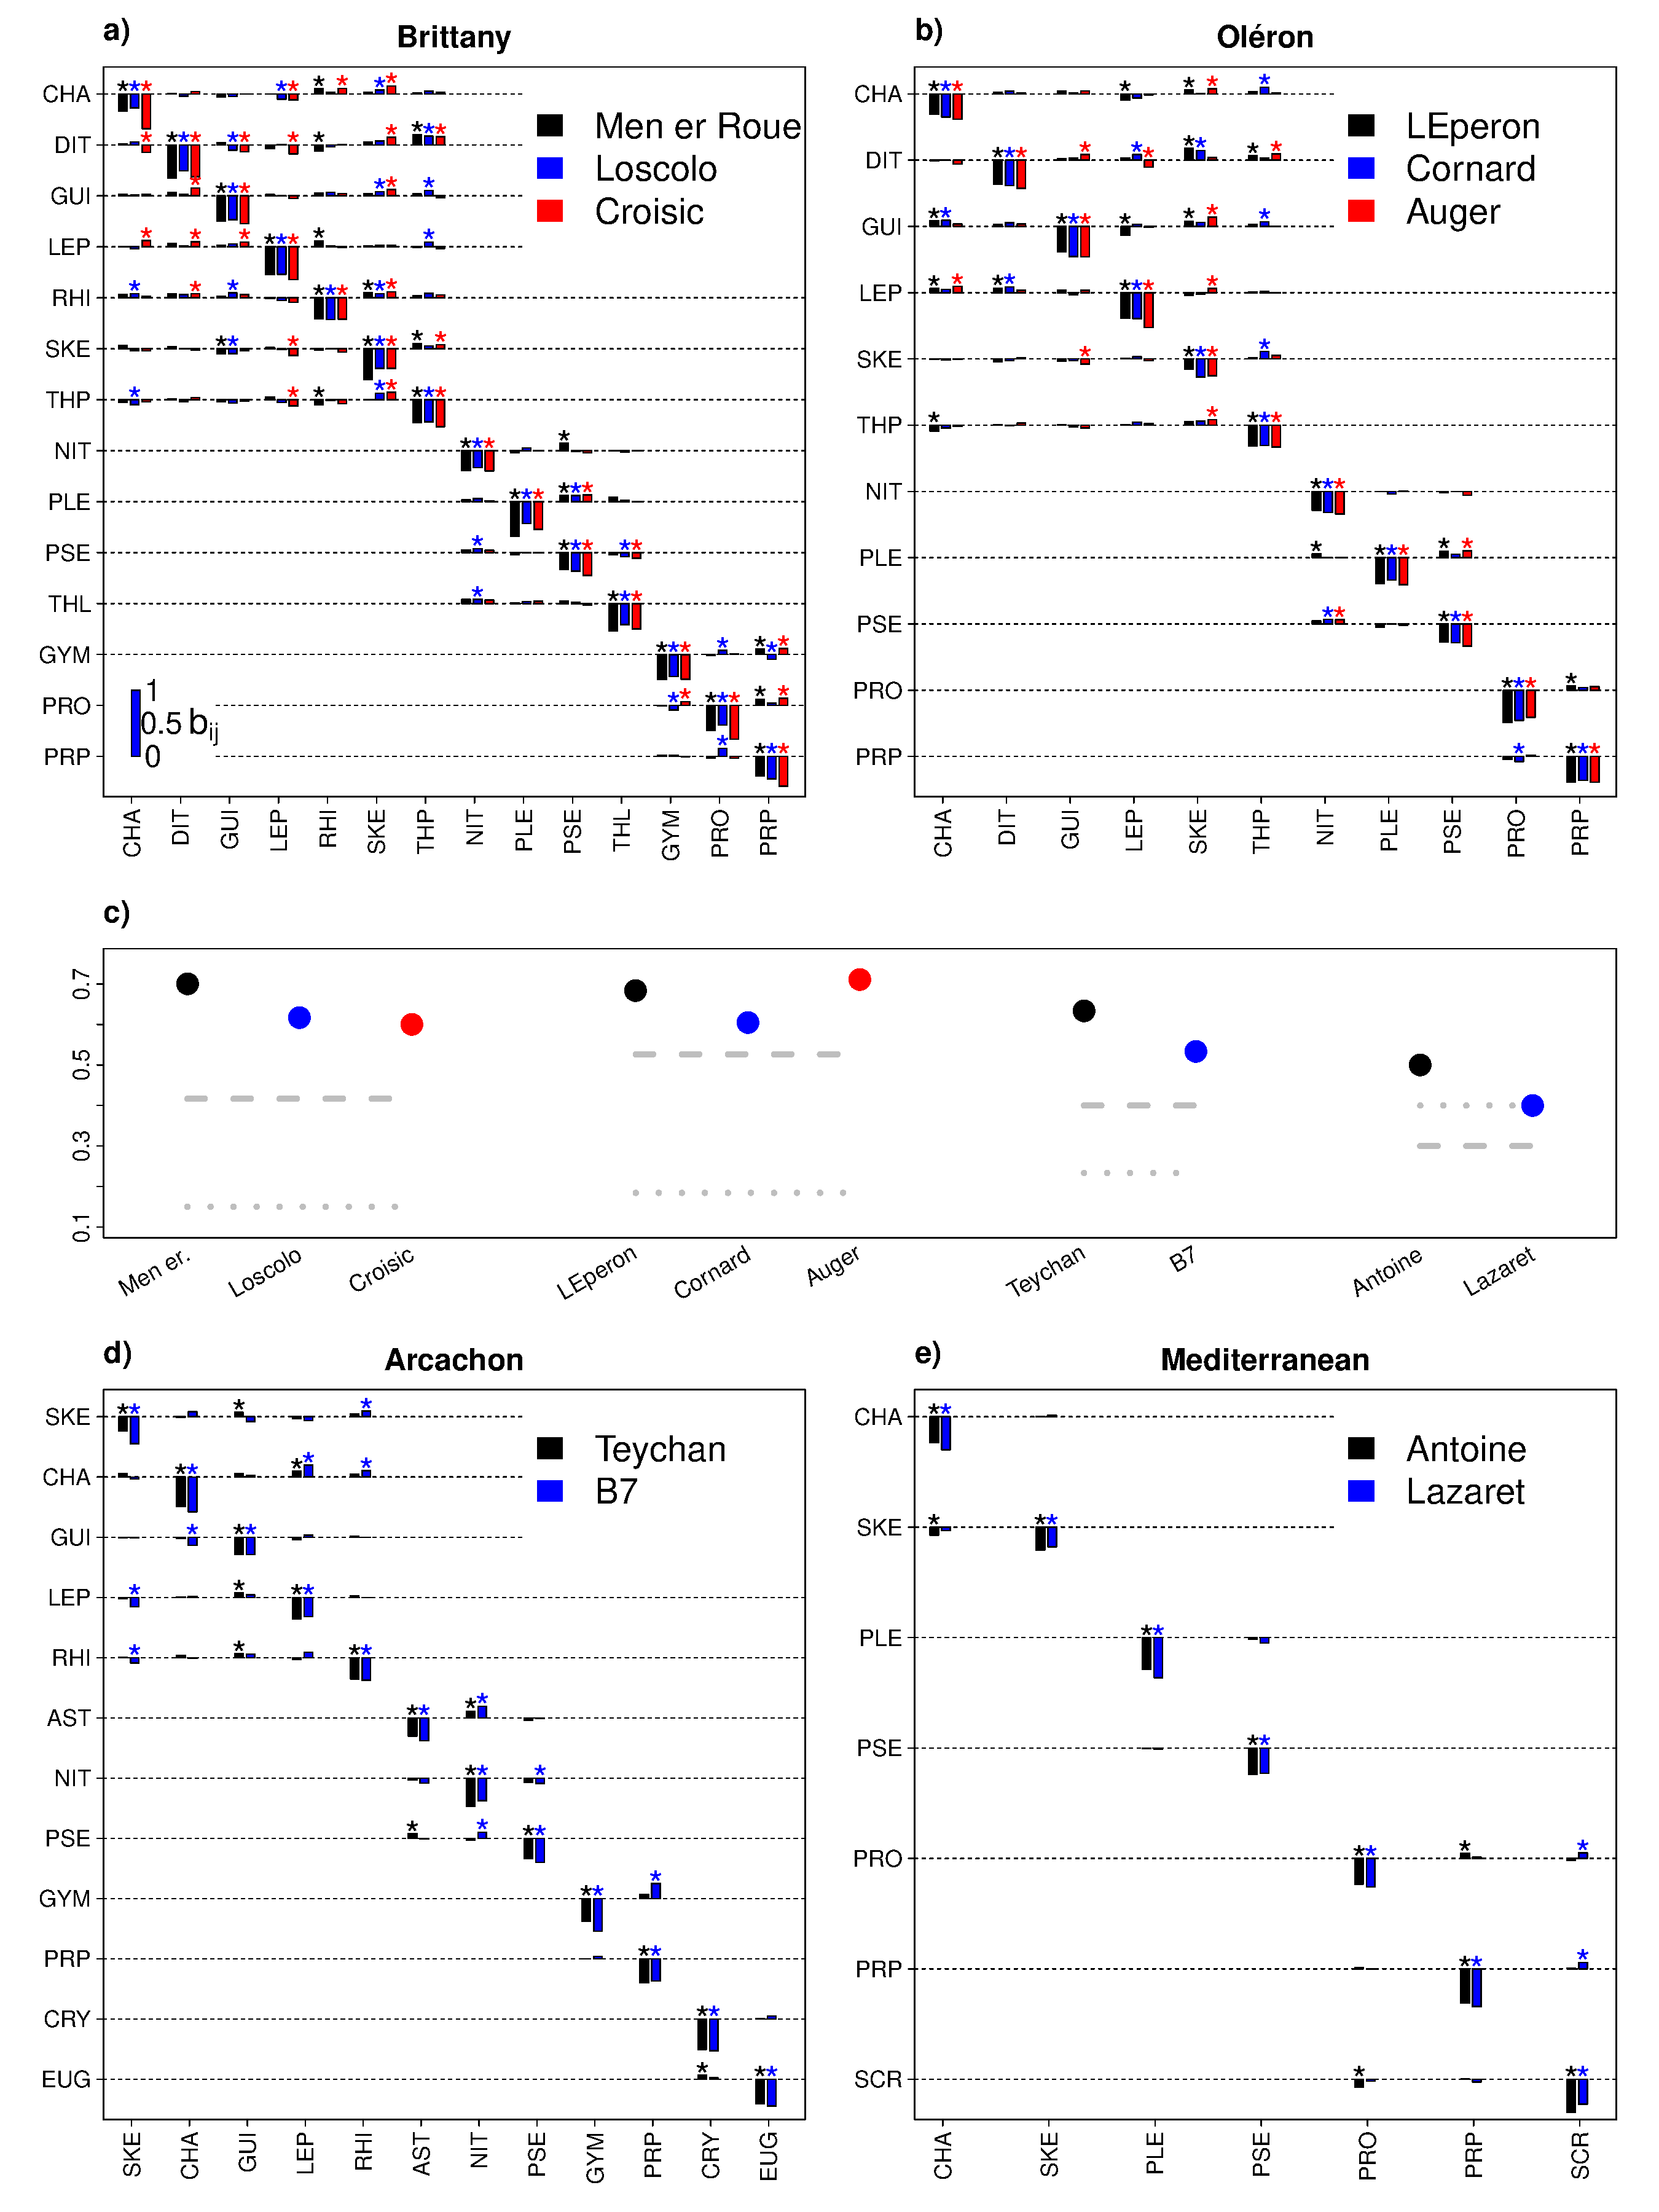
\includegraphics[width=0.767\textwidth]{biotic_interaction_matrices_MainFig_allin1_v4}
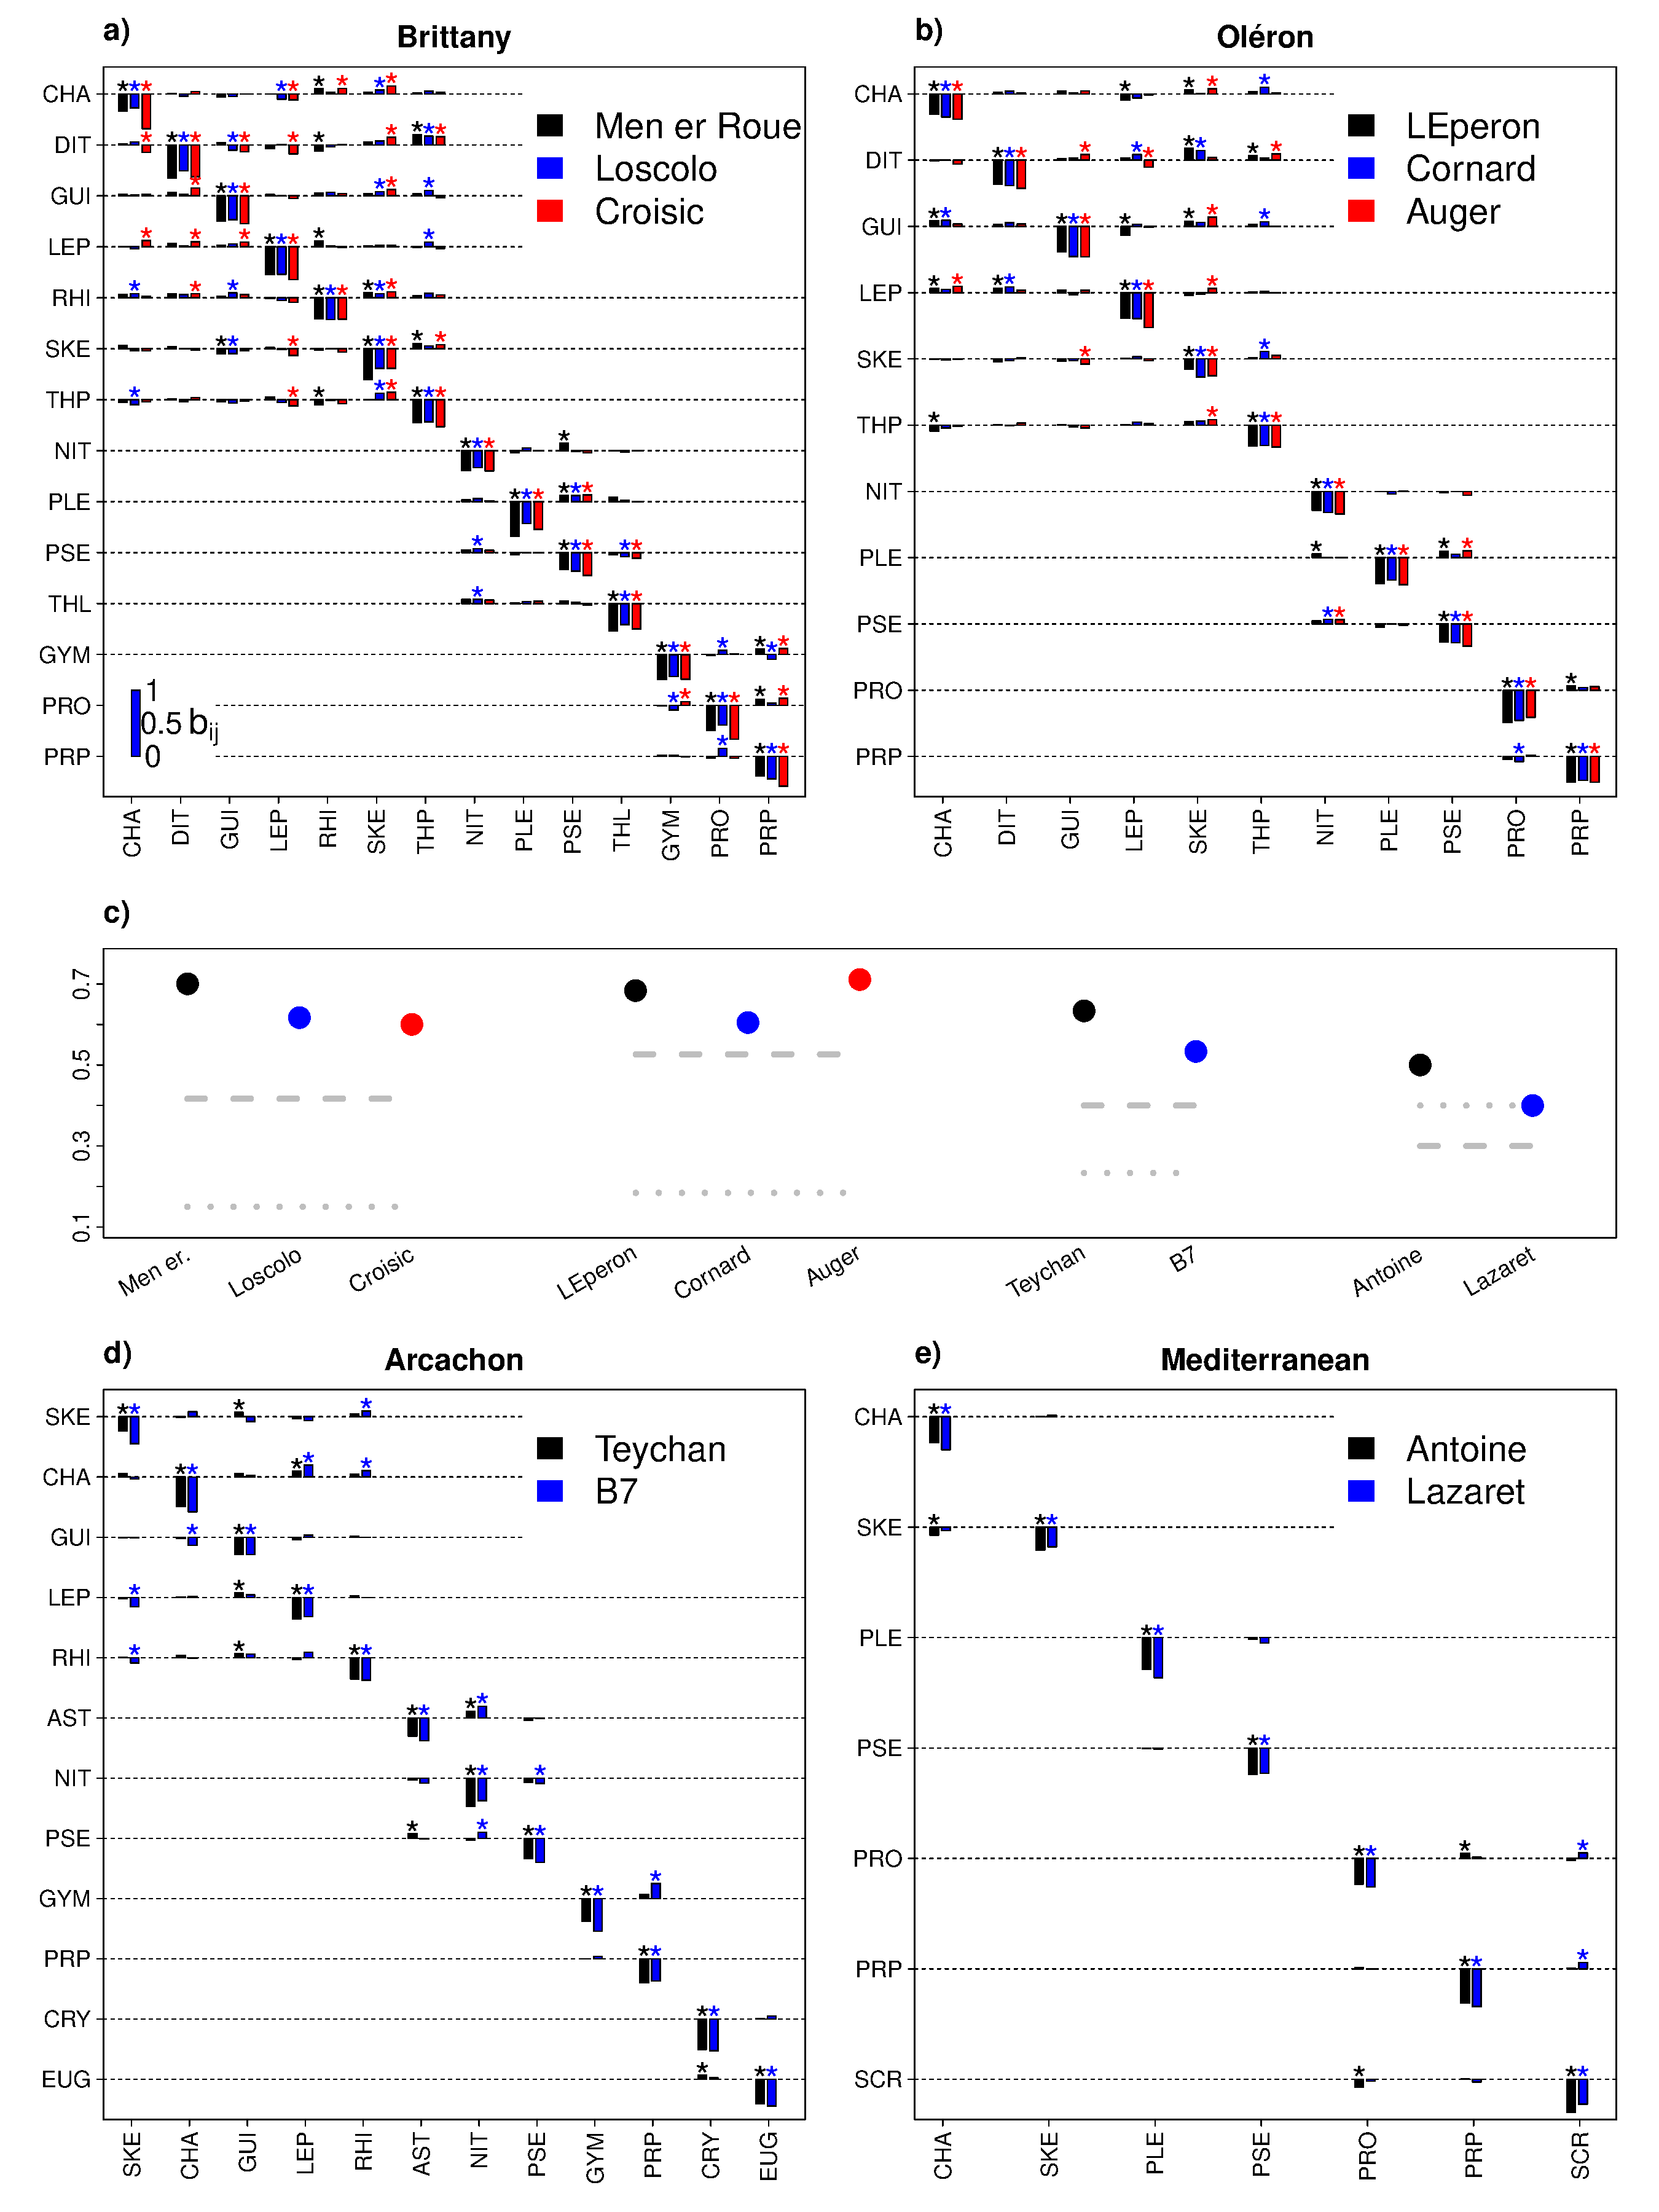
\includegraphics[width=0.85\textwidth]{biotic_interaction_matrices_MainFig_allin1_v4} %biorxiv version
\caption{\textbf{Interaction matrices estimated in 10 sites along the French
coastline}. Taxon $j$ (in columns) has an effect on taxon $i$'s growth rate (in rows) proportional to the bar height, which corresponds to the $\mathbf{B}-\mathbf{I}$ matrix (community composition in Table~S2, most parsimonious interaction scenario presented). The scale for the coefficient values is given at the bottom left of panel
a). Coefficients significantly different from 0 ($\alpha = 5\%$) are marked by asterisks ({*}). The fraction of positive interactions in each matrix is given by points in c) while the dashed (resp., dotted) line represents the ratio of interactions remaining positive (resp., negative) for all sites of a given region.}
\label{fig:Interaction-matrices}
\end{figure}

%Four regions are distinguished: Brittany (a), Oléron (b),
% Arcachon (d) and the Mediterranean Sea (e). Only interactions within
% a clade (pennate and centric diatoms, dinoflagellates, other planktonic
% taxa) are allowed, as this is the best fitting interaction scenario
% (Fig~S3). Taxon $j$ (in columns) has an effect on taxon $i$'s growth
% rate (in rows) proportional to the bar height. We present the interaction
% matrix minus the identity matrix ($\mathbf{B}-\mathbf{I}$) because
% this compares unambiguously intra- and intergenera interactions.

Using MAR(1) autoregressive models, we produced interaction matrices
\citep{ives_estimating_2003,hampton2013quantifying} -- i.e., Jacobian
community matrices on the logarithmic abundance scale \citep{ives_estimating_2003}.
Best-fitting models corresponded to a phylogenetically-structured
interaction scenario, where interactions only occurred betwen closely
related genera (Fig.~S3). This led to sparse, modular matrices that
have two main features. First, we observed a strong self-regulation
for all sites (Fig.~\ref{fig:Interaction-matrices}, diagonal elements
of all matrices), a feature that we had previously highlighted in
a more detailed analysis on one of the considered study regions \citep{barraquand_coastal_2018}.
The ratio of mean intragenus to intergenus interaction coefficients
varied between 6 and 10, not counting coefficients set to 0 before the
estimation process. When we included the zeroes in the interaction
matrix in the computation of the intra/inter mean interaction strength (see the Supporting Information for details of that computation),
the ratio rose to 21-43. Therefore, intragenus interactions were on average one order of magnitude stronger than intergenus interactions.

Second, although the percentage of facilitative interactions varied
among sites (between 40\% and 71\% of interactions in the selected
models), facilitation remained predominant in 9 sites out of 10 (only
Lazaret, in the Mediterranean Sea, has 60\% negative interactions).
Our observational setup being nested, with sites within regions, we
could examine whether locally positive interactions remain positive
in a regional context: the percentage of consistently positive interactions
at the regional level varied between 30\% and 53\%, higher than the
percentage of similarly defined negative interactions (between 15\%
and 40\%), except for sites in the Mediterranean Sea.

We found that the percentage of true mutualism (+/+) was substantial:
averaged over all sites, 32\% of all interactions were (+/+) while
only 12\% of them were (-/-), see also Fig.~S5. The sign correspondence
was not always maintained between regions: the only interaction that
was non-zero in the 10 sites (CHA/SKE) was mutualistic in Men er Roue
only (Brittany) and mixed (+/-) in all other sites. Within the same
region, however, interactions measured in different sites tended to
keep the same sign. In the 3 sites of Oléron, for instance, there
were 4 interactions which remained positive for both taxa involved
(CHA/GUI, DIT/GUI, LEP/THP, SKE/THP), 3 of them being also mutualistic
in some of the Brittany sites. This contradicts previous observations
that mutualistic interactions tend to be more context-dependent than
competitive interactions \citep{chamberlain_how_2014}.

\subsection*{Interaction network analysis}

The stability (\emph{sensu} resilience, \citealt{ives_stability_2007})
of all interaction matrices was not strongly affected by the percentage
of positive interactions or the mean and variance of the intergenus
interactions (Fig.~\ref{fig:Stability-community}). There was a slight
increase in stability with weighted connectance, with a drop in eigenvalue
modulus for weighted connectances between 0.09 and 0.1. The maximum
modulus of the interaction matrix eigenvalues remained between 0.65
and 0.80.

\begin{figure}[!ht]
%\centering 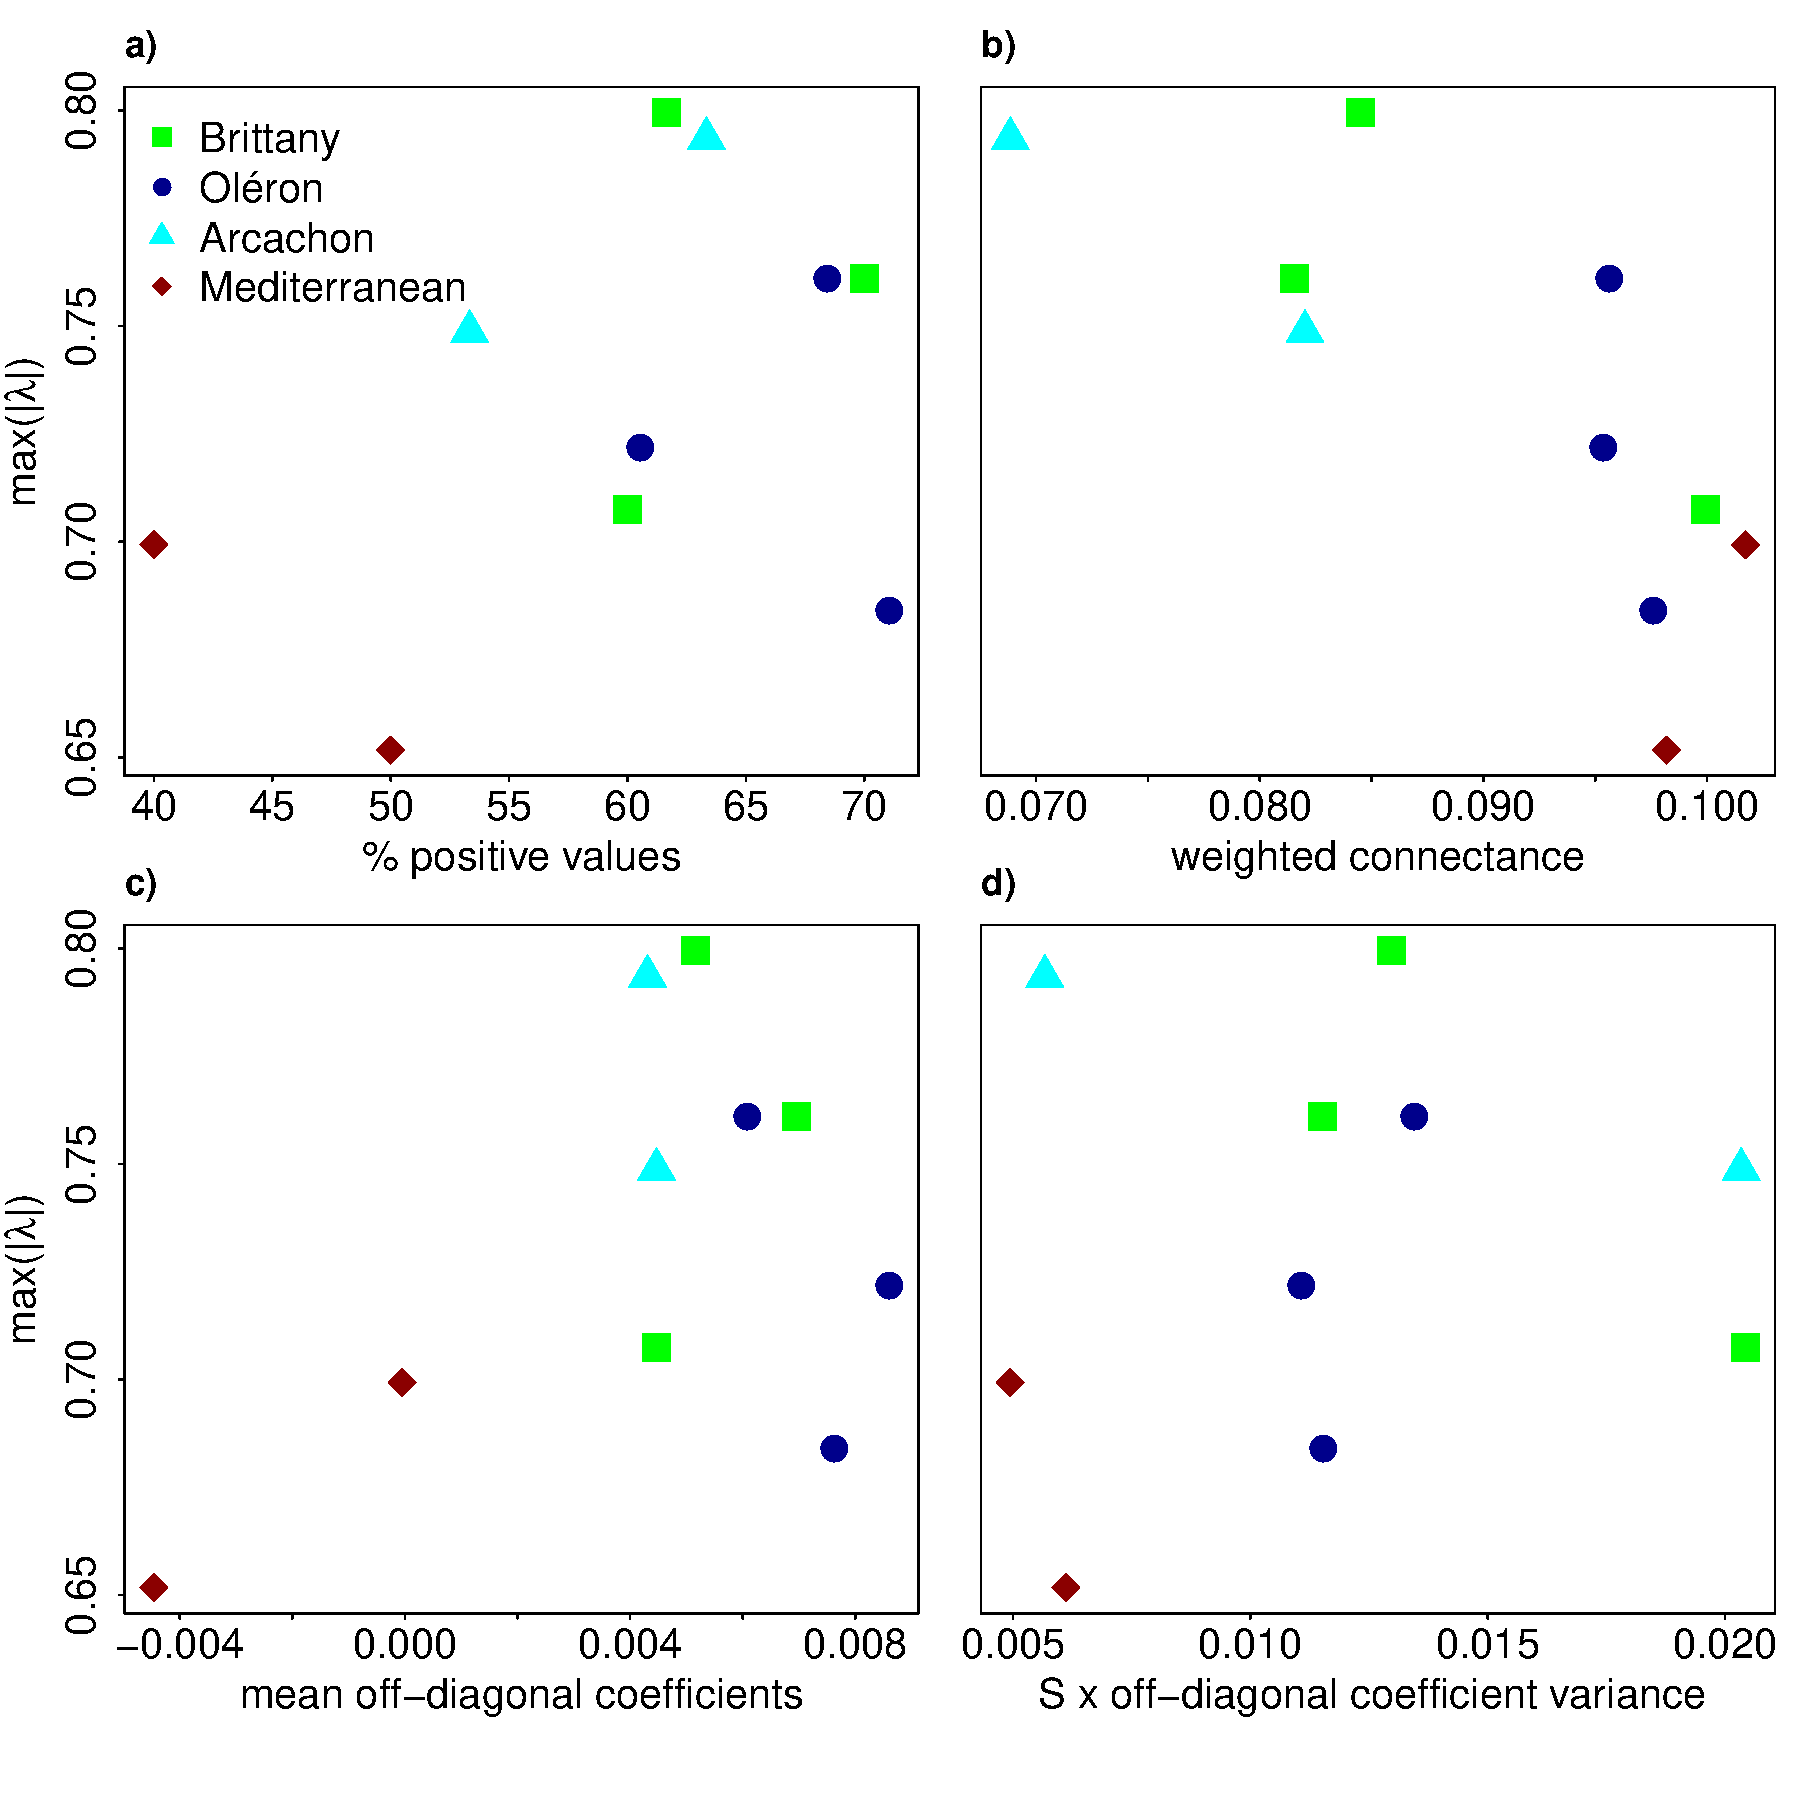
\includegraphics[width=1\textwidth]{complexity_stability_MainFig_pencenjustB_with_E_and_SV_with0}
\centering 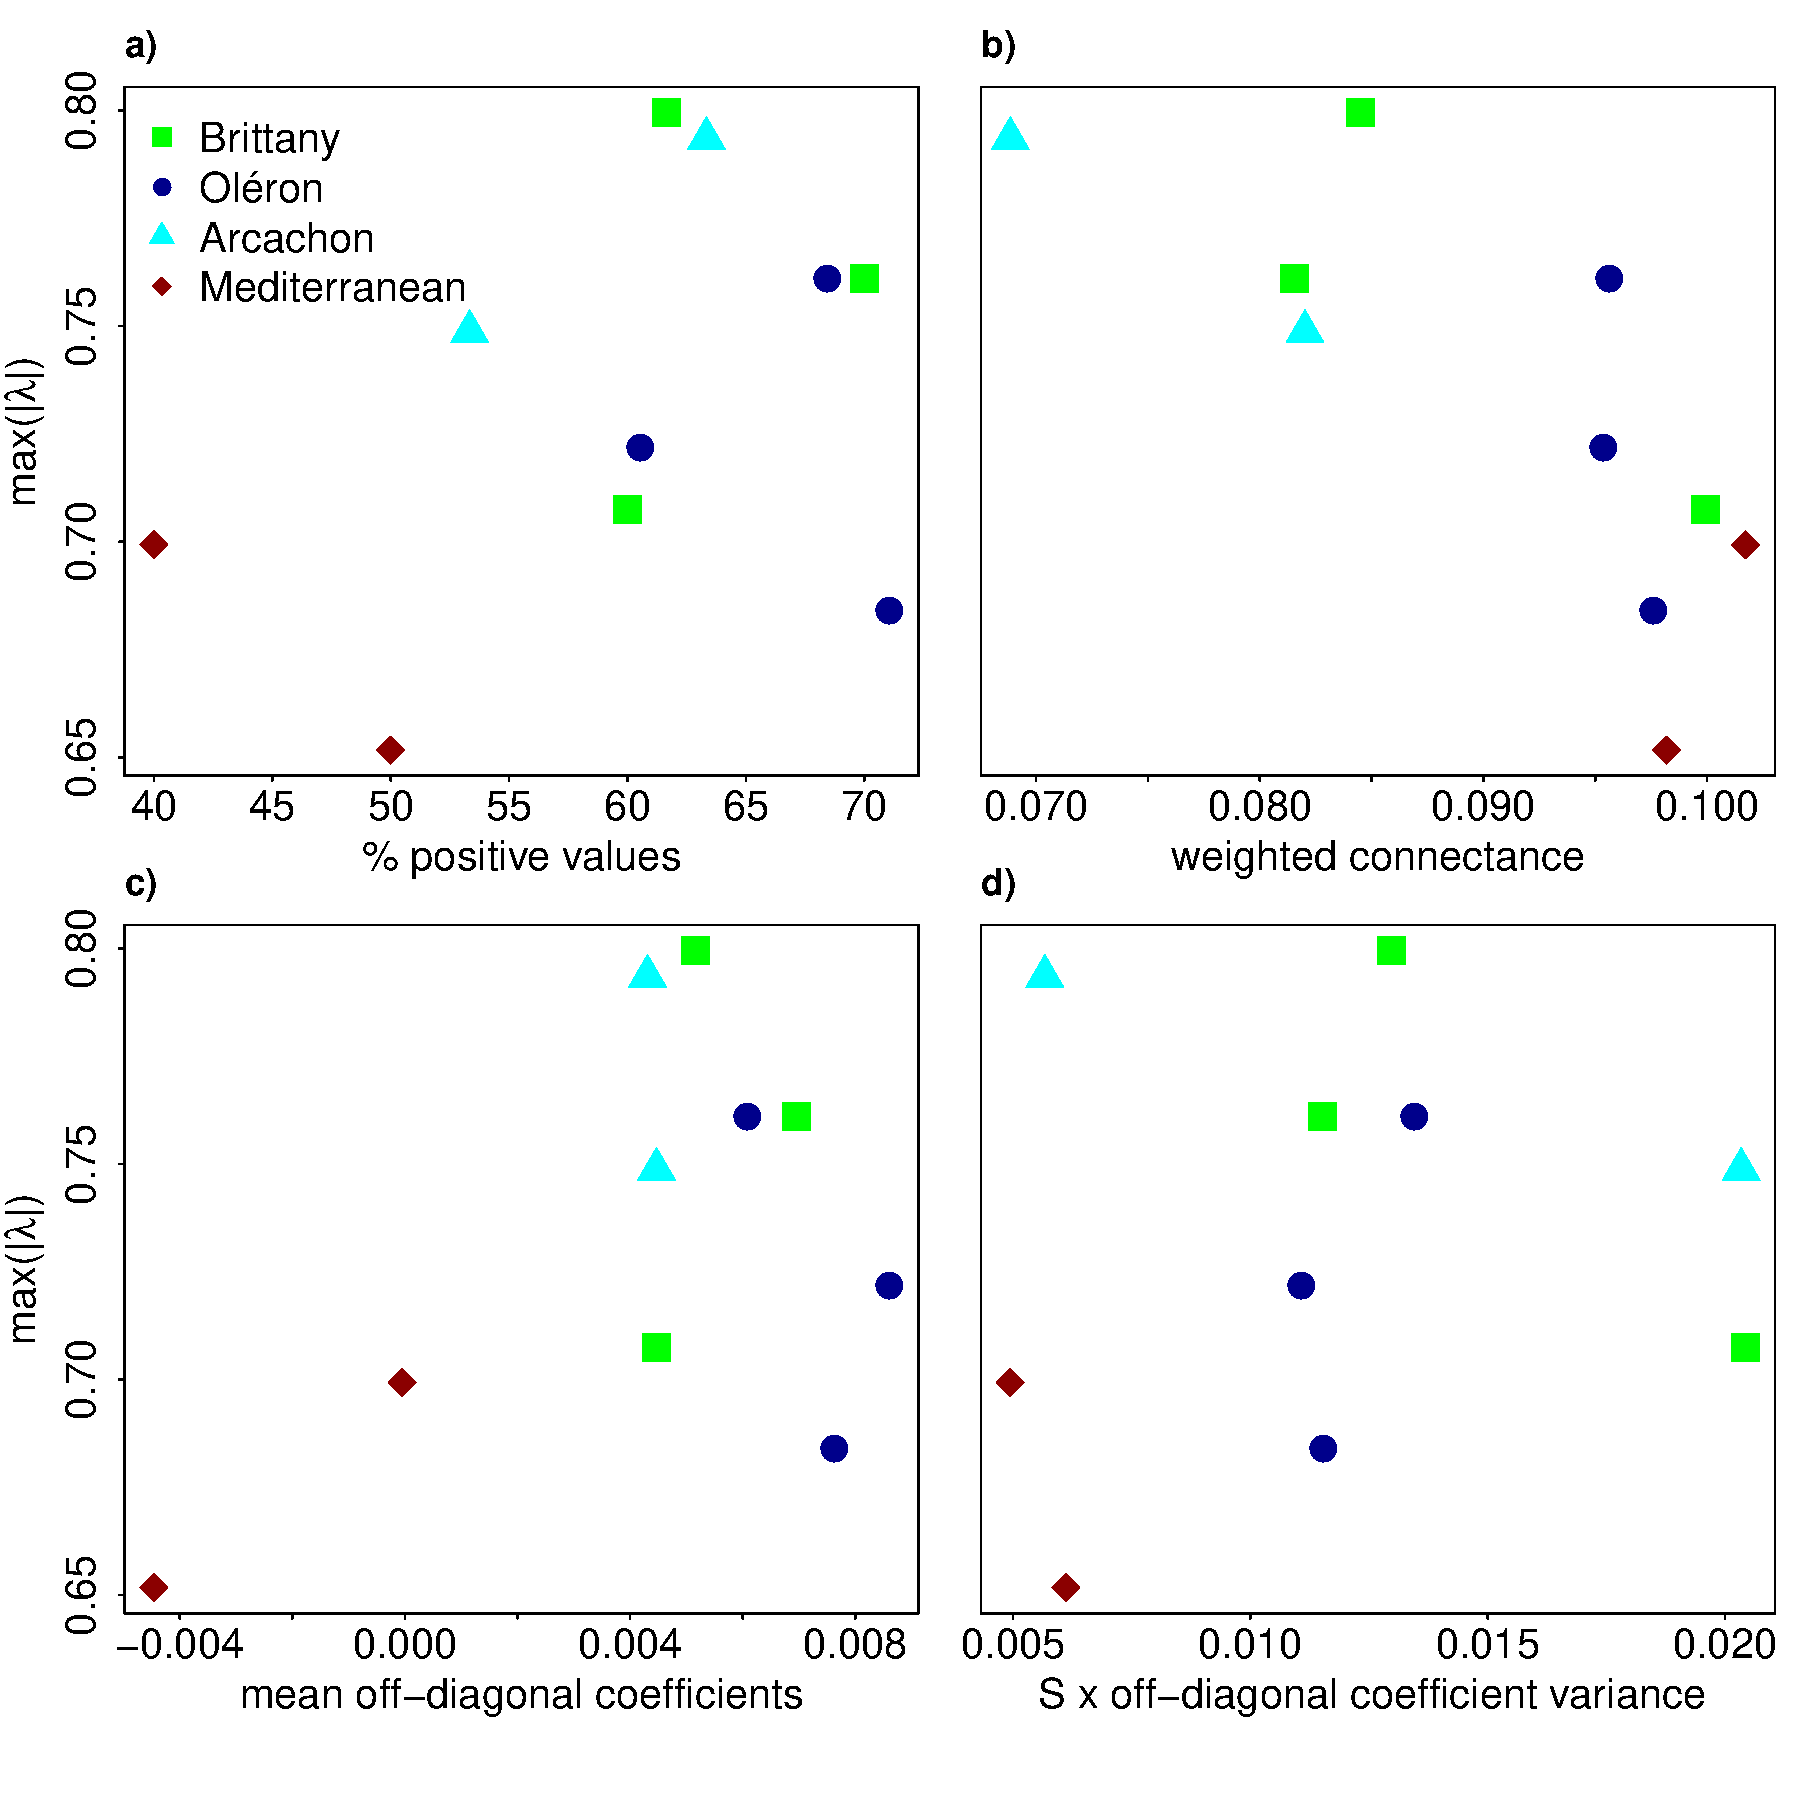
\includegraphics[width=0.8\textwidth]{complexity_stability_MainFig_pencenjustB_with_E_and_SV_with0} %biorxiv
\caption{\textbf{Relation between stability and complexity of the interaction
networks.} The maximum modulus of the eigenvalues of the interaction
matrix $\mathbf{B}$ indicates stability \emph{sensu} resilience. Off-diagonal coefficient variance is multiplied by the dimension of the network, that is the number of species in the region.
Each color or shape corresponds to a given region. The formula for
weighted connectance is given in the Supporting Information.}
\label{fig:Stability-community} 
\end{figure}

\begin{figure*}[!ht]
\centering{}\centering 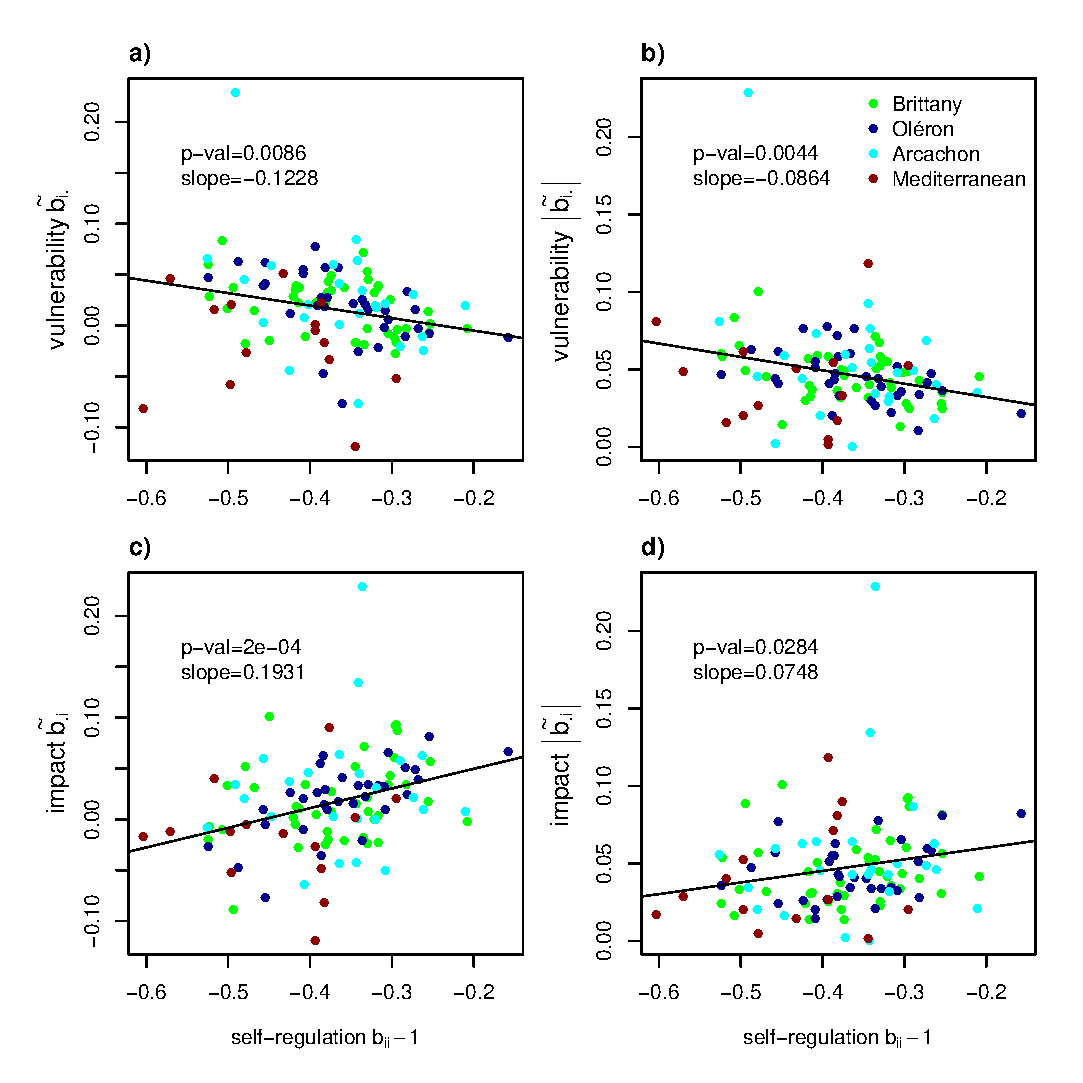
\includegraphics[width=1\textwidth]{pencen_generality_vs_vulnerability_MainFig}
\caption{\textbf{Relation between vulnerability/impact and self-regulation.}
Average vulnerability (effects of others on the focal taxon growth
rate, a-b) and impact (effects of the focal taxon on others' growth
rates, c-d), as well as self-regulation, are computed for untransformed
(a-c) or absolute (b-d) values of the coefficients of the interaction
matrix ($\mathbf{B}-\mathbf{I}$) for the 10 study sites. Each color
corresponds to a given region (Fig~S1). Linear regressions are shown
as black lines.}
\label{fig:Vulnerability_impact} 
\end{figure*}

Given that a direct complexity-stability (\textit{sensu} resilience)
link was not obvious, we investigated whether the matrix coefficients
had some particular structure that could help theoretical ecology
to make better null models of joint community dynamics and interactions
\citep{james_constructing_2015}. We defined two scores, vulnerability
(summed effect of others on the focal taxon growth rate, eq.~S5)
and impact (summed effect of the focal taxon onto other taxa's growth
rates, eq.~S6). Relations between inter- and intra-genus interactions
emerged (Fig.~\ref{fig:Vulnerability_impact}): genera that were
more self-regulating also had also a higher vulnerability score and
a lower impact score. Those two influences are likely to trade-off:
a high degree of self-regulation somehow buffers the effect of outside
influences on population dynamics. Taxa that were less self-regulating
were also more likely to have a stronger effect onto other taxa. As
these genera tended to be more abundant (Fig.~S7), this could be mediated
by the average density of a genus. It is important to note, however,
that these trends are weak and there is therefore a considerable amount
of randomness dominating the interaction matrix: many scenarios of
self-regulation vs limitation by others are therefore possible.

Aside from the trade-offs of Fig. \ref{fig:Vulnerability_impact},
we found no remarkable patterns of covariation between matrix elements (Fig.~S5)
other than a mean-variance scaling of interaction coefficients (Fig.~S6).

\subsection*{Literature comparison}

\begin{figure*}[!h]
%\centering 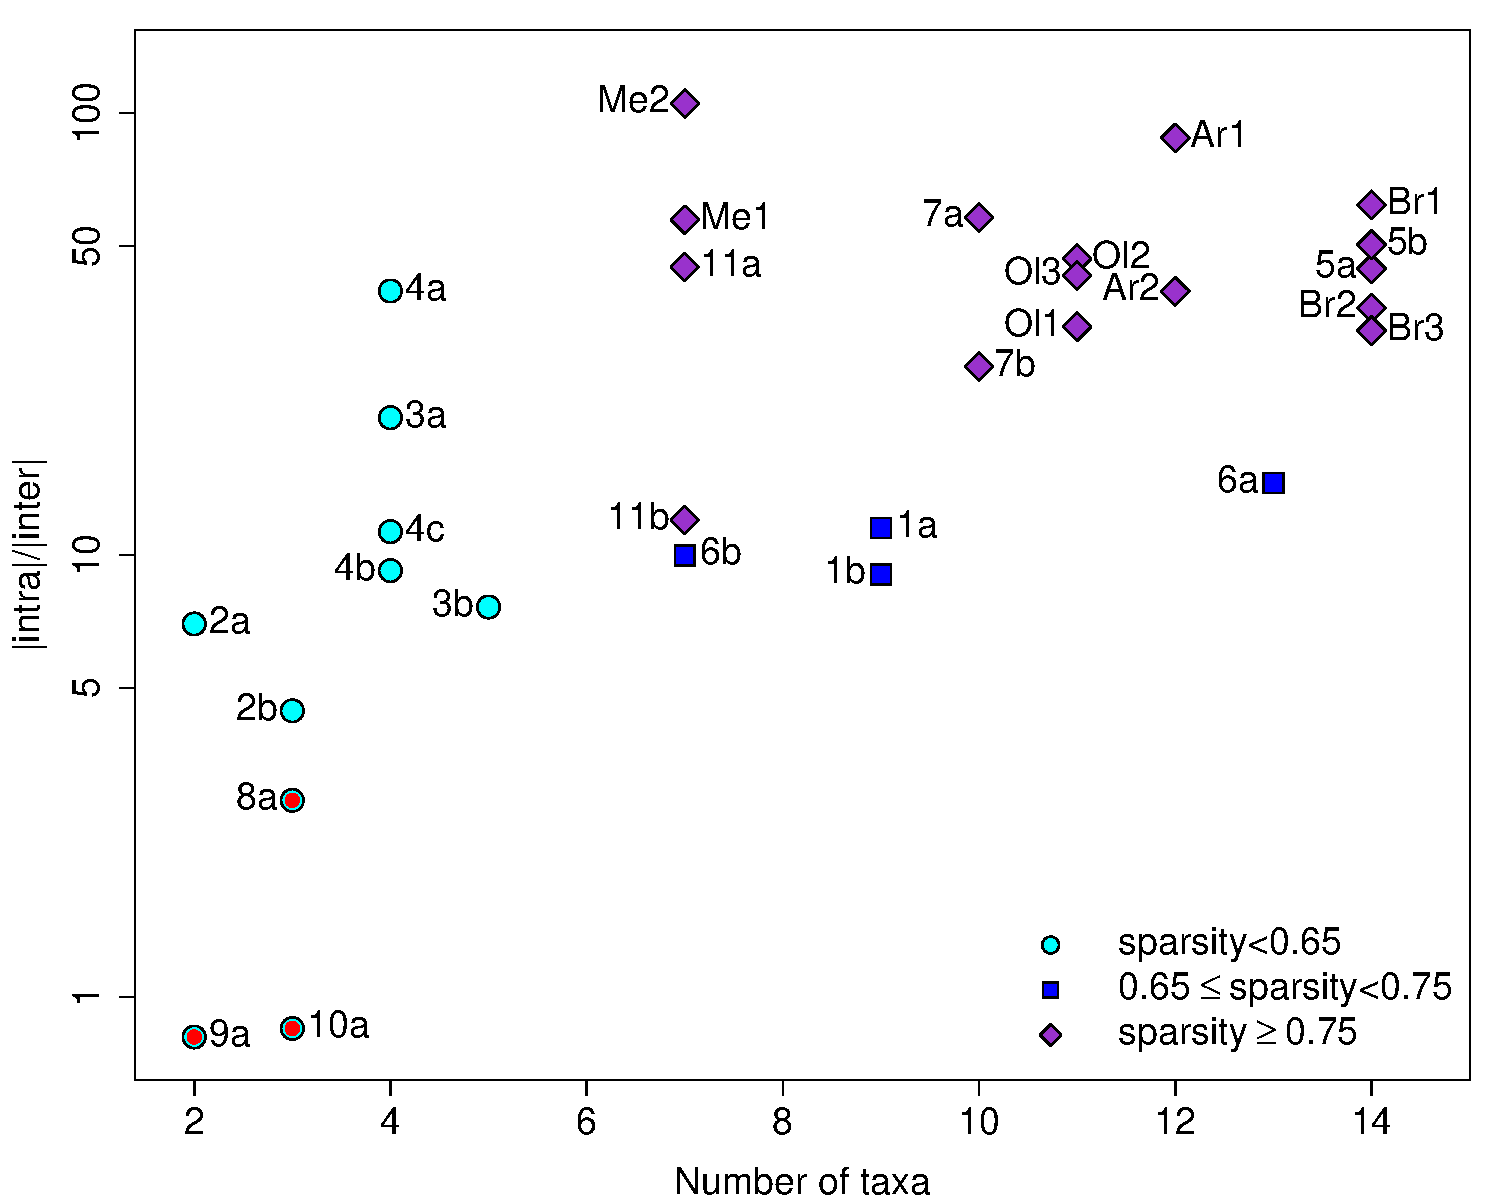
\includegraphics[width=0.8\linewidth]{Ratio_function_dim_tmp_withoutBarraquand_et_al_2018}
\centering 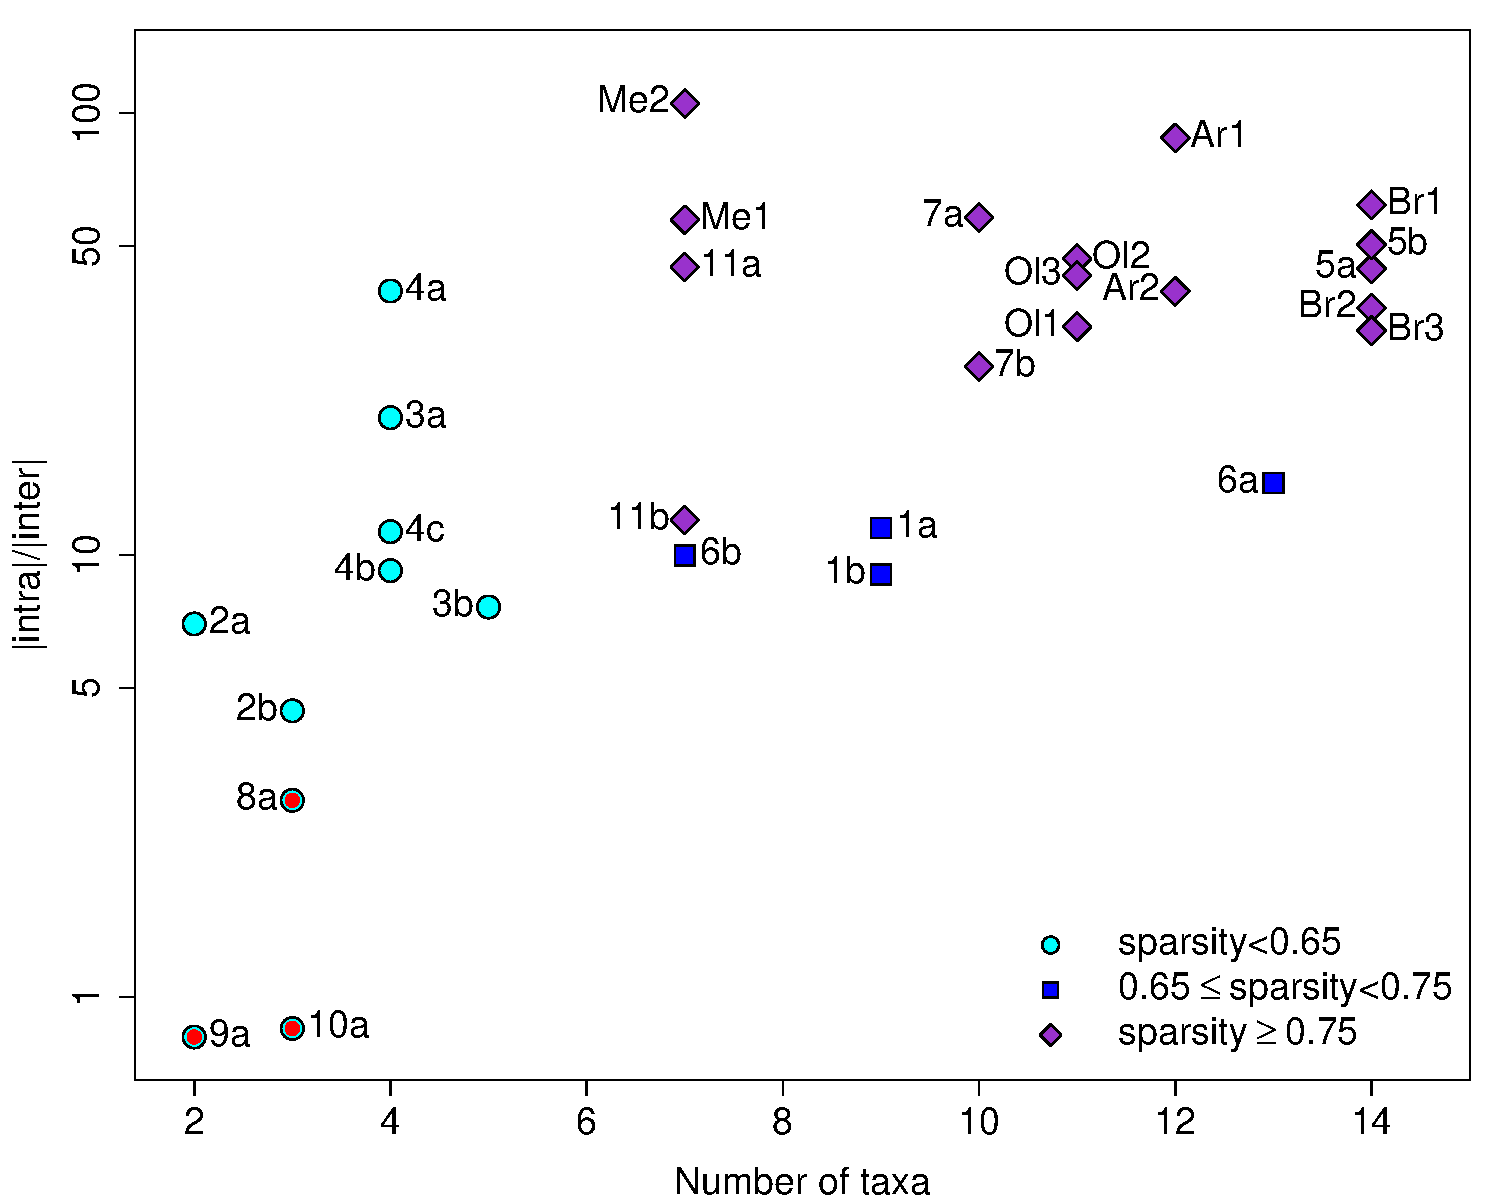
\includegraphics[width=0.75\linewidth]{Ratio_function_dim_tmp_withoutBarraquand_et_al_2018} %biorxiv
\caption{\textbf{Ratio of intra- to inter-group interaction strength in Multivariate
AutoRegressive (MAR) models.} The reference for each study is given
in Table~S4. Codes beginning with letters correspond to the present
study (Ar: Arcachon; Ol: Oléron; Br: Brittany; Me: Mediterranean Sea).
The symbol color and shape correspond to the sparsity of the interaction
matrix (e.g., the proportion of null interactions in the matrix).
Red dots correspond to terrestrial and/or low dimension predator-prey
systems, giving a lower bound for the intra/inter ratio. Intergroup
interactions were set to 0 when they were not specified in the articles
(in most cases, authors removed non-significant interactions at the
5\% level; Fig.~S9 is the same figure taking into account only
significant interactions)}
\label{fig:meta_ratio} 
\end{figure*}

Finally, we sought to put these results in a broader context by compiling
the intra vs inter group estimates of previous MAR(1) studies of long-term
observational count data (listed in Table~S4). We found that the
order of magnitude of intra/inter interaction strengths considered
here is not particularly above those found for most planktonic systems
to which MAR(1) models have been fitted, considering that our systems
are relatively high-dimensional and that the higher the number of
taxa, the larger the intraspecific regulation \citep{barabas_self-regulation_2017}.
We included in Fig.~\ref{fig:meta_ratio} not only plankton studies
but also a couple of vertebrate or insect studies on less diverse
communities, where interactions are stronger, in order to provide
lower bounds for the intra/inter ratio. The conclusion from this comparison
seems to be that, unlike small communities that can be tight-knit,
any diverse field system of competitors and facilitators has evolved
large niche differences making on average intragroup competition much larger
in magnitude than intergroup interactions.

\section*{Discussion}

\subsection*{Strong self-regulation and facilitation}

We found very large niche differences between genera, translating
into much higher intragenus than intergenus effects on growth rates
(i.e., strong self-regulation), together with a high degree of facilitative
net interactions.

The intra/intertaxa interaction strength ratio \citep{levine_importance_2009}
that we found, from 6--10 to above 20, depending on whether one includes interactions
set to zero before the estimation process, could appear very high
in light of previous intra/interspecific competition strength estimates
of 4 to 5 by \citet{adler_competition_2018}.  
Additional estimates using the unconstrained interaction matrix yielded ratios between 8 and 11 depending on the site (Table S3 and Fig. S8 in the Supporting Information), but weak intertaxa effects are likely to be inflated in the full model. Therefore, 
a intra/inter ratio of 10 seems like a conservative estimate, twice that of \citet{adler_competition_2018} 
who use a different model, i.e., a Lotka-Volterra competition model. We outline how to relate a MAR(1) model to a discrete-time Lotka-Volterra equivalent in the Supporting Information; even though there is a relationship between intra/inter ratios in both models, the relationship is not trivial when abundances vary greatly between species. Hence, to some degree, intra/inter ratios can differ between model frameworks or ways of measuring density-dependencies (e.g., a high measurement error due to using proxies of densities for plants can result in bias in interaction coefficient estimates, \citealp{detto_bias_2019}). However, a ratio intra/inter at least twice larger than the ones previously found may call for other explanations.
One could also argue that our high intra/inter ratio arises because we consider the genus as our baseline taxonomic unit, rather than the species. It is logical that niche differentiation increases as one gets up the phylogenetic tree, and that getting down
to the species level could slightly decrease that ratio (but see \citealp{narwani_ecological_2017},
in which phylogenetic closeness decreases competition strength). However, taxonomic resolution is unlikely to be the sole explanation for the high intra/inter ratio of interaction strength found here, for two reasons. First, phytoplankton species belonging
to different genera are often found to compete in experiments \citep{titman_ecological_1976,tilman_phytoplankton_1982,descamps-julien_stable_2005}. In the field-based dataset studied here, the same genera that are
considered in experiments are found not to compete (or only weakly),
hence there must be some niche differentiation occurring in the field
but not in the lab. Second, the only other study that managed to provide
MAR(1) estimates down to the species level for phytoplankton, that
of \citet{huber_role_2006}, provides an intra/interspecific strength
ratio similar to ours (point 7a in Fig.~\ref{fig:meta_ratio}). Strong
self-regulation seems therefore a genuine feature of field phytoplanktonic
communities. We discuss below possible mechanistic interpretations. 

Another main finding of our study is the large frequency of positive
interactions, with 30\% truly mutualistic (+/+) interactions and between
40 and 70\% facilitative effects. Although a seasonal environment
can generate some positive covariation between taxa, those effects
have already been filtered out by the inclusion of our 2 abiotic covariates
(Fig.~S4). The facilitative effects shown here are therefore residual
effects, once abiotic trends are accounted for. Between 40 and 70\%
facilitation can be compared to the meta-analysis by \citet{adler_competition_2018}
who also found facilitative interactions, but less than here ($\approx$30\%).
However, \citet{adler_competition_2018}'s review contains many experiments
while the plant literature is replete with field examples of facilitation
\citep{brooker_facilitation_2008,mcintire2014facilitation}, so that
plant facilitation could be higher in the field. At the moment, it
is therefore unknown how the predominance of facilitative interactions
that we found in phytoplankton compares to facilitation in terrestrial
plants. We note that several authors using MAR(1) models previously
forbade positive interactions within the same trophic level, so that
the fraction of facilitative interactions in plankton cannot be computed
from literature-derived MAR(1) estimates.

The large niche differences and facilitative interactions that arise
when considering a single trophic level are an emergent property,
resulting from hidden effects of resource or predator partitioning/sharing
\citep{chesson_updates_2018}. In our previous publication investigating
in detail the Arcachon study sites \citep{barraquand_coastal_2018},
we have argued that for phytoplankton, the strong intragroup density-dependence
could arise from effects of natural enemies \citep{haydon_pivotal_1994}.
Natural enemies could also very well create apparent mutualism between
prey species \citep{abrams_apparent_1998,de_ruiter_emergent_2017}.
We believe this to be likely for the present study, given that the
study regions (Arcachon, Oléron, Brittany, Mediterranean) have similar
predators (zooplankton, \citealp[e.g.,][]{jamet_zooplankton_2001,moderan_zooplankton_2010,tortajada_network_2012})
and parasites (viruses, \citealp[e.g.,][]{ory_pelagic_2010}; fungi).
Though natural enemies are good candidates to explain the observed
niche differences and emerging facilitation, one must bear in mind
that other known drivers of phytoplankton dynamics such as allelopathy
\citep{felpeto_allelopathy_2018}, auxotrophy \citep{tang_most_2010}
or hydrodynamics \citep{levy_role_2018} can all, in theory, help
create different niches and an emerging facilitation (see last subsection
of the Discussion). Finally, resources that are usually considered
limiting for all species might in fact not always be: \citet{burson_competition_2018}
show that phytoplanktonic taxa specialize on different components
of the light spectrum. This constitutes an example of fine-scale resource
partitioning of one resource, light, that all species and genera are
usually thought to compete for.

\subsection*{No complexity-stability relationship but connections between self-regulation
and intergroup interactions}

There was no relation between the complexity of the communities (measured
as either the weighted connectance or the interaction coefficient
variance) and their stability (measured
by the largest modulus of the eigenvalues, which quantifies
the return time to a point equilibrium, i.e., resilience). This result
is conditional upon our model being a good approximate description
of the system (i.e., no multiyear limit cycles or chaotic attractors
as the mapping between eigenvalues and actual stability is distorted
in that case, \citealp{certain_how_2018}). However, we already showed
on a subset of this data that a fixed point in a MAR(1) model, perturbed
by seasonality and abiotic variables, is an accurate description of
the system \citep{barraquand_coastal_2018}. Therefore, we are confident
that the absence of complexity-resilience relationship found here
is not a mere artefact of an inadequate model. This absence of direct link between
complexity and stability could be an actual feature of empirical systems,
as shown previously by \citet{jacquet_no_2016} using a different
technique. This result seems to contradict theory based on random
matrices, especially for competitive and/or mutualistic networks \citep{allesina_stability_2012}.
However, one must bear in mind that such result could also be generated by the limited size of our networks,
as random matrix theory relies on asymptotics \citep{allesina_stabilitycomplexity_2015}.
We should also mention that our interaction matrices (based on a discrete-time
model) are not strictly analogous to the ones used most frequently in theoretical ecology (continuous-time model), 
though the spectral radius (largest modulus) is here tightly related to the real part of the lead eigenvalue 
in equivalent continuous-time models (see Supporting Information). 
Thus while the jury is still out regarding the absence of complexity-resilience relation found here, it
may well be a genuine absence. In addition to complexity metrics,
we also found that the percentage of mutualistic interactions, that
is thought to affect the stability of a network, either positively
or negatively \citep{mougi2012diversity,coyte_ecology_2015,garcia2018effect},
does not in fact have a major impact on our networks' resilience.

In addition to weighted connectance and interaction variance, indices
at the genus level (vulnerability and impact) approximate the average
effects exerted and sustained by any given taxa in the different study
sites. While, at the network level, network structure (either complexity
measures or the percentage of mutualistic interactions) did not affect
resilience, a relation emerged between self-regulation, necessary
for coexistence, and genus-level indices. We found that the more a
genus is self-regulated, the more it tends to be vulnerable to other
genera's impacts and the less it impacts other genera. We examined whether
vulnerability and impact could be affected by phylogenetic correlations;
they were not, as on Fig.~\ref{fig:Vulnerability_impact}, points
were not clustered according to genus, family or phylum. High self-regulation
usually indicates large niche differences with the rest of the community,
and it makes therefore sense that a species/genus whose needs strongly
differ from the others only marginally impacts the resources of the
other coexisting species. This is what we expect under strong niche
partitioning. A low self-regulation was also correlated with
high average abundance, which echoes findings by \citet{yenni_persistent_2017}
who demonstrated that rare species usually show stronger self-regulation.
This correlation between relative rarity and self-regulation could
explain the lesser impact of highly self-regulated species/genus:
a taxon which dominates the community composition can have a major
effect on the others, especially as they usually cover more space,
while it is harder for the less common taxa to have large impacts.
In contrast, it was more difficult to explain the relationship between
self-regulation and vulnerability: a genus that is more self-regulated
and less common was found here to be on average more vulnerable to
other genera's increases in densities. Such relation implies greater
stability (\emph{sensu} resilience, \citealt{ives_estimating_2003},
and also invariability, \citealt{arnoldi2019multidimensionality})
for the network as a whole, because the taxa that are the more vulnerable
to other taxa's impacts are also those whose dynamics are intrinsically
more buffered. By which mechanisms this could happen is so far unclear
and open to speculation. It could just be a ``mass effect'': common
taxa are in high enough numbers to deplete resources or change the
environment in ways that affect the less common ones, but the reverse
is not true. As a final note on relationships between interaction matrix coefficients, 
we caution that the trends evidenced are all relatively weak:
considerable stochasticity still dominates the distribution of interaction
matrix coefficients.

\subsection*{Ghosts of competition past and present}

Overall, the dominance of niche differentiation in observational plankton
studies -- based on our analysis of the REPHY dataset and re-analysis
of the MAR(1) literature -- is similar to what has been recently
found in plant community studies \citep{volkov_patterns_2007,adler_competition_2018}
or empirically parameterized food webs including horizontal diversity
\citep{barabas_self-regulation_2017}. Large niche differences might
be due to the ghost of competition past, i.e., competition has occurred
in the past, leading to strong selection and subsequent evolution,
and then to progressive niche separation. In this scenario, species
have evolved niches that allow them not to compete or to interact
only weakly (very strong facilitative effects might be likewise destabilizing,
\citealp{coyte_ecology_2015}). The likely predator effects that we
highlighted above could be comprised within such niche differentiation
\emph{sensu largo}: specialized predators can make strong conspecific
density-dependence emerge \citep{bagchi_pathogens_2014,comita_testing_2014},
while switching generalists can also promote diversity \citep{vallina2014maximal}.
Both predators and resources have often symmetrical effects and can
therefore contribute almost equally to such past niche differentiation
\citep{chesson_updates_2018}.

An intriguing new possibility, dubbed the ``ghost of competition
present'' \citep{tuck_strong_2018}, suggests by contrast that spatial
distributions in relation to abiotic factors might have a large impact
on the interaction strengths inferred from temporal interaction models
such as ours. Recent combinations of model fitting and removal experiments
have shown that model fitting usually underestimates the effect
of competitors that are uncovered by removal experiments \citep{tuck_strong_2018,adler_weak_2018}.
This could occur for instance if species are spatially segregated
(at a small scale) because each species only exists within a domain
where it is relatively competitive (Pacala's spatial segregation hypothesis, chapter 15 in 
\citealt{pacala1997biologically}), while a focal species could spread
out if competitors were removed. This means that a species can be
limited by competitors, but act so as to minimize competition (a little
like avoidance behaviour in animals) and maximize opportunities for
positive interactions, which implies that competition is in effect
hard to detect when all species are present. This mechanism would require some spatial
segregation between phytoplankton species at the scale of interactions,
i.e., at the microscale. At the moment, while it is known that fine-scale
hydrodynamics generate inhomogeneities at the microscale \citep{barton_impact_2014,breier_emergence_2018}
it is yet quite unclear how they might affect multivariate spatial patterns
of species distributions (\textit{sensu} \citealt{bolker_spatial_1999}
or \citealt{murrell_heteromyopia_2003}). Moreover, even with some microscale spatial segregation between
species, a ``ghost of competition present'' mechanism might not work in phytoplankton as in terrestrial plants, 
because the turbulent, ever-changing aquatic environment imposes additional constraints on the spatial distribution of organisms.

\subsubsection*{Acknowledgements}

This study was only made possible by the dedication of the members of the REPHY program by Ifremer \citep{REPHY_db}, providing invaluable
data through years of fieldwork. We are grateful to David Murrell for his careful reading and suggestions, and to Peter Adler for helpful exchanges. We also want to thank Bérangère Péquin for constructive comments, as well as Gyuri Barabás whose thoughtful suggestions improved the connection made to continuous-time stability theory. This study was supported by the French ANR through LabEx COTE (ANR-10-LABX-45).

\subsubsection*{Supporting Information}
This article contains supporting information.

\subsubsection*{Authors' contributions}
CP and FB contributed equally to the project design and the methodology. The computer code was written by CP. The authors jointly interpreted the results and co-wrote the manuscript after an early draft by FB.

\subsubsection*{Data accessibility} The REPHY dataset has already been published
\citep{REPHY_db}. All scripts for MAR models and subsequent network analyses
are available online in a GitHub repository (\url{https://github.com/CoraliePicoche/REPHY-littoral}).

\nolinenumbers \bibliographystyle{methods}
\bibliography{phytoInteractions_ref}
 %\bibliography{bib_fig_review}
\end{document}
